
\section{Automatic Topic Labeling}
\label{kap:automaticTL}
%Topics are multinomial distributions a set of recurring themes that are discussed in the collection.

%Topics are a set of recurring themes that are discussed in the collection and represent as a multinomial distribution. Often the top words of the distribution is taken to represent

%of topic modeling can be used. Topic models refer to a set of algorithms that discoverthe topics or hidden thematic structure in a collection of documents. A topic modeltakes a set of documents as the input and outputs topics, a set of recurring themesthat are discussed in the collection, and the degree to which each document expressthese topics (Blei, 2012b). The results of the topic modeling algorithms can be usedto organize, visualize, summarize, and understand large collections of documents.

%A topic is commonly understood to be a a phrase or subject that best describesthe content of a text. In contrast, in topic modeling, every topic is a probabilitydistribution over all words in the collection of documents. In each topic a differentset of words has a high probability and we visualize the topic by listing the mostprobable terms.

Topic Models are used to discover latent topics in a corpus to help to understand large collections of documents. These topics are multinomial distributions over all words in a corpus. Normally the top terms of the distribution are taken to represent a topic but these words are often not helpful to interpret the coherent meaning of the topic. Especially, if the person is not familiar with the source collection.
With the help of Automatic Topic Labeling (\ac{ATL}) we want to reduce the cognitive overhead of interpreting these topics and therefore facilitate the interpretation of the topics.
Of course, the topics can be labeled manually by domain experts but this method is time consuming if there are hundreds of topics. Additionally, the topic labels can be biased towards the users opinion and the results are hard to replicate. \\
%%TODO human turks?
We are working with domain specific data dealing with organic food. To generate meaningful labels we can not make use of human turks but we need domain experts who are proficient in this area. Therefore we submitted the topics to our domain experts to label them. But only 50 of the generated topics for each dataset were handed in, in order to not burden them, since this process is very time-consuming. The datasets were labeled by three labelers who tried to find a suitable label, which captures the meaning of the topic and is easily understandable. After labeling every dataset the three labels were compared and a final label was set. If at least two labelers had the same label, this was taken as the final one. If the given labels were not comparable, no label was set at all. \\
To relieve our domain experts in the following chapter two approaches of \ac{ATL} are described. In Section \ref{sec:intrinsic} an intrinsic method was used, which is only working on texts and topics from our datasets to generate the labels according \cite{Mei2007}. Section \ref{sec:extrinsic} describes an extrinsic approach by using a lexical database for the English language called \textit{Wordnet} to label the topics.
 
%The domain experts labeled our topics. There were three labelers who tried to find a suitable label, which captures the meaning of the topic and is easily understandable. After labeling every dataset the three labels were compared and a final label was set. If at least two labelers had the same label, this was taken as the final one. If the given labels were not comparable, no label was set at all.\\


\subsection{Related work}                                                
\label{sec:relWorl: atl}
\textit{\cite{Lau2011}} generated a label set out of the article titles which were found in Wikipedia or Google by searching the top N words from the topics, called primary candidate labels. Afterwards, these were chunkized and n-grams were generated, which were searched in Wikipedia and Google. Theses secondary candidate labels were then filtered with the \textit{related article conceptual overlap} (RACO), that removed all outlier labels, like stop words. Then the primary and secondary candidate labels were ranked by features like \ac{PMI}, used for measuring association, and the student’s t test. The results were measured with the mean absolute error score for each label, which is an average of the absolute difference between an annotator’s rating and the average rating of a label, summed across all labels. The score lay between 0.5 and 0.56 on a scale from 0 to infinity.

On topics from Twitter \textit{\cite{Zhao2011}} used  a topic context sensitive Page Rank to find keywords by boosting the high relevant words to each topic. These keywords were taken to find keyword combinations (key phrases) that occur frequently in the text collection. The key phrases were ranked according to their relevance,i.e. whether they are related to the given topic and discriminative, and interestingness, the re-tweeting behavior in Twitter. To evaluate the key words Cohen’s Kappa was used to calculate the iterrater reliability between manually and automatically generated key phrases. The Cohen’s Kappa coefficient was in the range from 0.45 to 0.80, showing good agreement.

\textit{\cite{Allahyari2015}} created a topic model OntoLDA which incorporates an ontology into the topic model and provides \ac{ATL} too. In comparison with \ac{LDA}, OntoLDA has an additional latent variable, called concept, between topics and words. So each document is a multinational distribution over topics, each topic is a multinomial distribution over concepts and each concept is a multinomial distribution over words.  Based on the semantics of the concepts and the ontological relationships among them the labels for the topics are generated in followin steps:
\begin{description}
	\item (1) construction of the semantic graph from top concepts in the given topic
	\item (2) selection and analysis of the thematic graph (subgraph form the semantic graph)
	\item (3) topic graph extraction from the thematic graph concepts
	\item (4) computation of the semantic similarity between topic and the candidate labels of the topic label graph
\end{description}
The top N labels were compared with the labeling from \textit{\cite{Mei2007}} by calculating the precision after categorizing the labels into good and unrelated. The more labels were generated for a topic the more imprecise they got but the preciser \textit{\cite{Mei2007}} labels were.

\textit{\cite{Hulpus2013}} made use of the structured data from DBpedia, that contains structured information from Wikipedia. For each word of the topic the Word-sense disambiguation (WSD) chose the correct sense for the word from a set of different possible senses. Then a topic graph was obtained form DBpedia consisting of the closest neighbors and the links between the correct senses. Assuming the topic senses which are related, lie close to each other, different centrality measures were used and evaluated manually to identify the topic labels. The final labels then were compared to textual based approaches and the precision after categorizing the labels into good and unrelated was calculated.

\cite{Kou2015} captured the correlations between a topic and a label by calculating the cosine similarity between pairs of topic vectors and candidate label vectors. CBOW, Skip-gram and Letter Trigram Vectors were used. The candidate labels were extracted from Wikipedia articles that contained at least two of the top N topic words. The resulting labels for the different vector spaces were compared to automatically generated gold standard labels, representing the most frequent chunks of suitable document titles for a topic. The final labels were ranked by human annotators,too, and were considered as a better solution than the first word of the top N topic words. 

For topics and preprocessed Wikipedia titles \textit{\cite{Bhatia2016}} used word and title embeddings for both, generated by either doc2vec(for fine-grained labels) or word2vec (for generic labels), to generate topic labels. The relevance of each title embedding was measured with the pairwise cosine similarity of the word embeddings for the top N topic words. The sum of of the relevance of doc2vec and vec2doc served as ranking for the labels. The results were evaluated the same way like in \cite{Lau2011}.

\textit{\cite{Magatti2009}} used a given tree-structured hierarchy from the Google Directory to generate candidate labels for the topics. These were compared with the topic words applying different similarity measures showing a coherent behavior with respect to the semantics of the compared concepts. The most suitable label was then selected by exploiting a set of labeling
rules. This approach is applicable to any topic hierarchy summarized through a tree. The resuts were promising.

\textit{\cite{Mei2007}} generated labels based on the texts collection and their related topics by chunking and building n-grams. They approximated the distribution for the labels and compared these to the distribution of the topic by calculating the \ac{KL} divergence. To maximize the mutual information between the label and the topic distributions the calculated divergence has to be minimized. Three human assessors measured the results and found out that the final labels are effective and robust although applied on different genres of text collections. 


\subsection{Intrinsic Topic Labeling}
\label{sec:intrinsic}
The intrinsic topic labeling is only based on the text collection and the extracted topics and does not use any external ontologies or embeddings. Because \textit{\cite{Mei2007}} were the only ones who generated topic labels by using an intrinsic approach, we decided to apply their \ac{ATL} on our data, using the implementation from Github\footnote{https://github.com/xiaohan2012/chowmein}. 

In their paper \textit{\cite{Mei2007}} consider noun phrases and n-grams as candidate labels and use \ac{POS}-tags to extract the label according to some grammar from the text collection. We apply the n-grams approach to select (NN - NN) or (JJ - NN) English and (NN -NN) or (ADJD - NN) German bi-grams as suitable labels for the topics.

The candidate labels were ranked by their semantical similarity to the topic model $\theta$. To measure the semantic relevance between the topic and the label \textit{l} a distribution of words \textit{w} for the label $p(w|l)$ was approximated by including a text collection \textit{C} and a distribution $p(w|l,C)$ was estimated, to substitute $p(w|l)$. Then the \ac{KL} divergence $D(\theta||l)$ was applied to calculate the closeness between the label and the topic distribution $p(w|\theta)$. So the \ac{KL} divergence served to capture how well the label fits to our topic. If the two distributions perfectly match each other and the divergence is zero we have found the best label. 
The relevance scoring function of \textit{l}  to $\theta$ is defined as the negative \ac{KL} divergence $-D(\theta||l)$ of $p(w|\theta)$ and $p(w|l)$ and can be rewritten as follows by including \textit{C}:
\begin{align}
\begin{split}
	Score(l,\theta) = &-D(\theta||l) =
	-\sum_{w} p(w|\theta)log\frac{p(w|\theta)}{p(w|l)}\\ =
	&-\sum_{w} p(w|\theta)log\frac{p(w|C)}{p(w|l,C)} -\sum_{w} p(w|\theta)log\frac{p(w|\theta)}{p(w|l)}\\ &-\sum_{w} p(w|\theta)log\frac{p(w|l,C)}{p(w|l)} \\ =
	&-\sum_{w} p(w|\theta)log\frac{p(w,l|C)}{p(w|C) p(l|C)} -D(\theta||C)\\ &-\sum_{w} p(w|\theta)log\frac{p(w|l,C)}{p(w|l)}\\  =
	&-\sum_{w} p(w|\theta) PMI(w,l|C)-D(\theta||C) + Bias(l|C) 
\end{split}
\end{align}
We can see that the relevance scoring function consists of three parts. The first part represents the expectation of \ac{PMI} $E_{\theta}(PMI(w,l|C))$ between \textit{l} and the words in the topic model given the context \textit{C}, the second part by the \ac{KL} divergence between $\theta$ and \textit{C} and the third part can be viewed as a bias using context
\textit{C} to infer the semantic relevance \textit{l} and $\theta$. This bias can be neglected for our data because we have used the same text collection for  producing the topics and the labels. The same applies to the second part, because the \ac{KL} divergence has the same value for all candidate labels. Therefore, we rank the topic labels with 
\begin{equation}
Score(l,\theta) = E_{\theta}(PMI(w,l|C))
\label{Mei:Scoring}
\end{equation}

\begin{figure}[t]
	\begin{minipage}[t]{0.5\textwidth}
		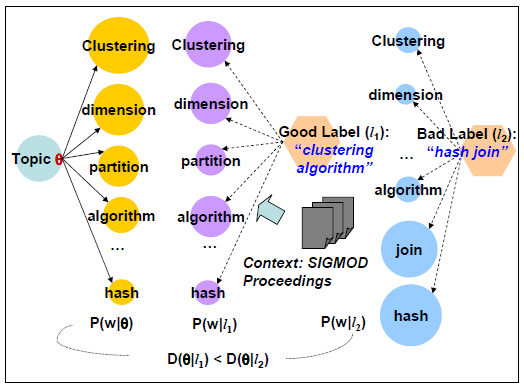
\includegraphics[width=\textwidth]{gfx/Mei/MeiGoodLabel.png}
	\end{minipage}
	\begin{minipage}[t]{0.512\textwidth}
		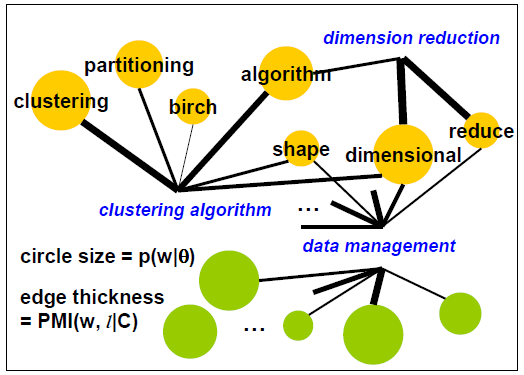
\includegraphics[width=\textwidth]{gfx/Mei/MeiScoring.png}
	\end{minipage}
	\caption[Relevance scoring function for \ac{ATL}]{Relevance scoring function for \ac{ATL}. Adapted from \cite{Mei2007}}
	\label{pic:ScoringFunction}
\end{figure}

The relevance scoring function is also described visually in Figure \ref{pic:ScoringFunction}. The circles represent the probability of terms. The larger the circle the higher is the probability. On the left one can see that the label with lower \ac{KL} divergence is the best one. To approximate $p(w|l)$ the \textit{SIGMOD Proceedings} were used as the text collection \textit{C}. Analogously, we used our datasets. On the right one can a weighted graph, where each node is a term in the topic model $\theta$ and the edges between terms and the label are weighted by their \ac{PMI}. The weight of the node indicates the importance of a term to the topic, while the weight of each edge indicates the semantical strength between label and term. The relevance scoring function ranks a node higher if the label has a strong semantic relation to the important topical words. Visually, this can be understood that the label is ranked higher if it connects to large circle by a thick edge.

So far only the labeling of a topic was considered, but a characteristic of a good label is the discrimination towards other topics in the topic model,too. It is not useful if many topics have the same labels, although it may be a good label for the topic individually, because we can not make differentiations between the topics. The label should have a high semantic relevance to a topic and low relevance to other topics. In order to take this property into account the $Score(l,\theta)$ in \ref{Mei:Scoring} was adjusted to: 
\begin{equation}
Score'(l,\theta_{i}) = Score(l,\\theta_{i}) - \mu Score(l,\theta_{1,...,i-1,i+1,...})
%Score(l,\theta) = (1+\dfrac{\mu}{k-1}) E_{\theta_{i}}(PMI(w,l|C)) - \dfrac{\mu}{k-1} \sum_{j=1...k} %E_{\theta_{j}}(PMI(w,l|C))
\end{equation}
$\theta_{1,...,i-1,i+1,...}$ describes all topics except the $\theta_{i}$ and $\mu$ controls the discriminative power.

%The semantic relevance function already guarantees that the label covers the maximal semantic information of $\theta$. Even though one label covers only a topic partially. So a selection of multiple labels for a topic shall cover different aspects of the topic. This is called the intra-topic coverage. For the selection of labels the Maximal Marginal Relevance (MMR) (\cite{Carbonell1998}) was used to get high relevant and low redundant labels.
\subsubsection{Evaluation}
We applied the \ac{ATL} according \cite{Mei2007} on the Dataset \ref{chris:daten}. 


 



%changed the implementation, used our preprocessing(stop words)
%made postagging on our data 
%without bigramms
%with bigrams
%with postags
%candidate label generation:

%	Code: Candidate phrase detection using pointwise mutual information: POS tag constraint can be applied. For now, only bigrams are considered.

%	Changes: 
%		-our vectorizer, 
%		nope-throw out words which are smaller then 3 characters
%		-used our preprocessing
%		- generated our own postags on the data
	
	
\subsection{Extrinsic Labeling}
\label{sec:extrinsic}

\footnote{http://www.nltk.org/howto/wordnet.html}
%

\textbf{Chapter \ref{sec:related}} \\[0.2em]
\blindtext
